\documentclass[tikz, border=10pt]{standalone}
\usepackage{amsmath,amssymb}

\begin{document}
	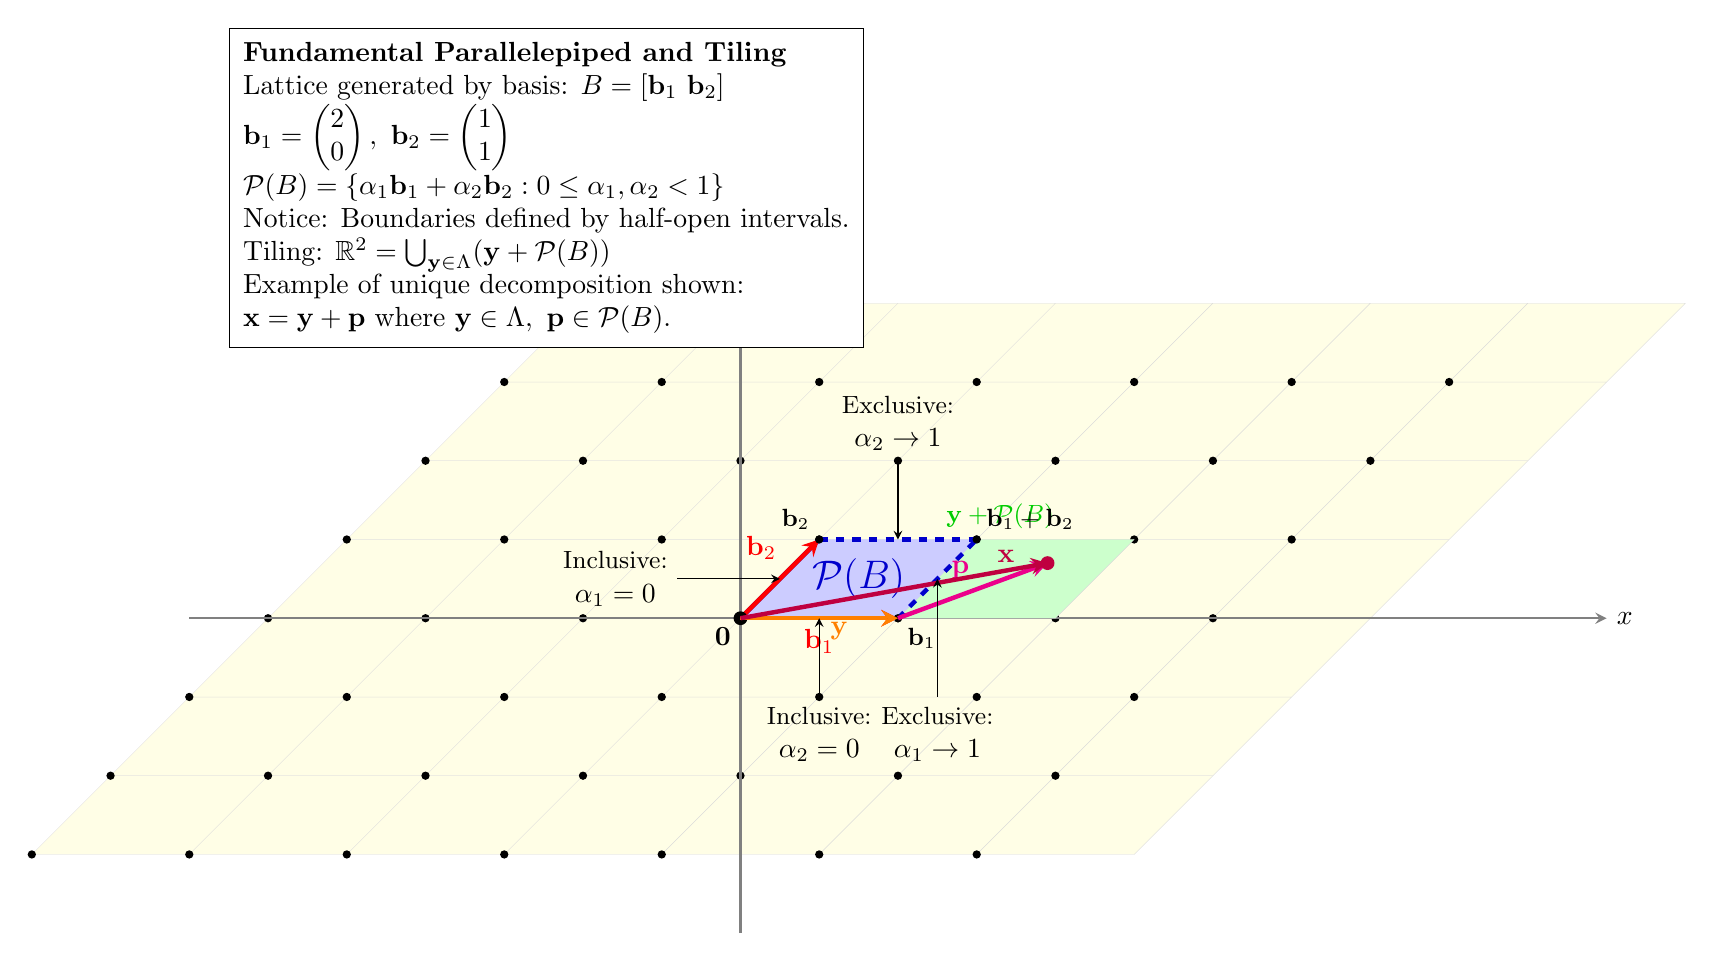
\begin{tikzpicture}[>=stealth]
		
		% Define reusable parallelogram path for tiling and context
		% based on vertices: O=(0,0), b1=(2,0), b1+b2=(3,1), b2=(1,1)
		\def\cellpath{(0,0) -- (2,0) -- (3,1) -- (1,1) -- cycle}
		
		% Define coordinates for unique representation example x = y + p
		\coordinate (X) at (3.9, 0.7);
		\coordinate (Y) at (2, 0);
		
		% ==========================================
		% LAYER 1: Tiling Copies of P(B)
		% ==========================================
		% Tiling range i, j in [-3, 3] to fill the visible plane
		\foreach \i in {-3, -2, -1, 0, 1, 2, 3} {
			\foreach \j in {-3, -2, -1, 0, 1, 2, 3} {
				% Calculate current lattice point y = i*b1 + j*b2
				\coordinate (Lpoint) at ({\i*2 + \j*1}, {\j*1});
				
				% Shade the translated copy y + P(B)
				\fill[yellow!10!white, draw=gray!30, line width=0.1pt, shift={(Lpoint)}] \cellpath;
				
				% Mark the lattice point
				\fill[black] (Lpoint) circle (1.5pt);
			}
		}
		
		% Draw standard axes, scaled to fit the tiling
		\draw[->, thick, gray] (-7,0) -- (11,0) node[right, black] {$x$};
		\draw[->, thick, gray] (0,-4) -- (0,7) node[above, black] {$y$};
		
		% ==========================================
		% LAYER 2: Fundamental Domain, Basis, and Decomposition
		% ==========================================
		
		% Highlight containing cell for the unique decomposition example point x = y + p
		\fill[green!20, draw=gray!30, line width=0.1pt, shift={(Y)}] \cellpath;
		\node[green!80!black] at ([xshift=1.3cm, yshift=1.3cm]Y) {\small $\mathbf{y} + \mathcal{P}(B)$};
		
		% Fill the fundamental parallelepiped P(B) at the origin with distinctive blue
		\fill[blue!20] \cellpath;
		
		% Draw the half-open boundaries on P(B)
		% Solid boundaries [0, ...) are inclusive:
		\draw[ultra thick, blue!80!black] (0,0) -- (2,0); % along b1 (alpha2=0)
		\draw[ultra thick, blue!80!black] (0,0) -- (1,1); % along b2 (alpha1=0)
		% Dashed boundaries (..., 1) are exclusive:
		\draw[ultra thick, blue!80!black, dashed] (2,0) -- (3,1); % far end along b1 (alpha1=1)
		\draw[ultra thick, blue!80!black, dashed] (1,1) -- (3,1); % far end along b2 (alpha2=1)
		
		% Draw and label the basis vectors b1, b2 from the origin
		\draw[->, ultra thick, red] (0,0) -- (2,0) node[midway, below] {$\mathbf{b}_1$};
		\draw[->, ultra thick, red] (0,0) -- (1,1) node[pos=0.6, above left] {$\mathbf{b}_2$};
		
		% Mark other vertices of the fundamental domain
		\fill[black] (2,0) circle (1.5pt) node[below right] {\small $\mathbf{b}_1$};
		\fill[black] (1,1) circle (1.5pt) node[above left] {\small $\mathbf{b}_2$};
		\fill[black] (3,1) circle (1.5pt) node[above right] {\small $\mathbf{b}_1+\mathbf{b}_2$};
		
		% Label the fundamental domain P(B)
		\node[blue!80!black, font=\bfseries] at ({2/2 + 1/2}, {0/2 + 1/2}) {\Large $\mathcal{P}(B)$};
		
		% Origin node with specific mark and label
		\fill[black] (0,0) circle (2.5pt) node[below left] {$\mathbf{0}$};
		
		% Visualize unique representation: x = y + p
		\draw[->, ultra thick, orange] (0,0) -- (Y) node[midway, below right, yshift=1mm] {$\mathbf{y}$};
		\draw[->, ultra thick, magenta] (Y) -- (X) node[midway, above left, xshift=1mm] {$\mathbf{p}$};
		\draw[->, ultra thick, purple] (0,0) -- (X) node[pos=0.8, above right] {$\mathbf{x}$};
		\fill[purple] (X) circle (2.5pt);
		
		% ==========================================
		% LAYER 3: Definitions and Boundary Logic
		% ==========================================
		
		\draw[<-] (1.0, 0) -- (1.0, -1.0) node[below, align=center] {\small Inclusive: \\ $\alpha_2=0$};
		\draw[<-] (0.5, 0.5) -- (-0.8, 0.5) node[left, align=center] {\small Inclusive: \\ $\alpha_1=0$};
		\draw[<-] (2.0, 1.0) -- (2.0, 2.0) node[above, align=center] {\small Exclusive: \\ $\alpha_2 \to 1$};
		\draw[<-] (2.5, 0.5) -- (2.5, -1.0) node[below, align=center] {\small Exclusive: \\ $\alpha_1 \to 1$};
		
		% Main Math Box
		\node[align=left, anchor=north west, fill=white, draw=black, inner sep=5pt] at (-6.5, 7.5) {
			\textbf{Fundamental Parallelepiped and Tiling} \\
			Lattice generated by basis: $B = [\mathbf{b}_1 \ \mathbf{b}_2]$ \\
			$\mathbf{b}_1 = \begin{pmatrix} 2 \\ 0 \end{pmatrix}, \ \mathbf{b}_2 = \begin{pmatrix} 1 \\ 1 \end{pmatrix}$ \\
			$\mathcal{P}(B) = \{\alpha_1 \mathbf{b}_1 + \alpha_2 \mathbf{b}_2 : 0 \le \alpha_1, \alpha_2 < 1\}$ \\
			Notice: Boundaries defined by half-open intervals. \\
			Tiling: $\mathbb{R}^2 = \bigcup_{\mathbf{y} \in \Lambda} (\mathbf{y} + \mathcal{P}(B))$ \\
			Example of unique decomposition shown: \\
			$\mathbf{x} = \mathbf{y} + \mathbf{p}$ where $\mathbf{y} \in \Lambda, \ \mathbf{p} \in \mathcal{P}(B)$.
		};
		
	\end{tikzpicture}
\end{document}